\documentclass[9pt]{cheatsheet}

\cheatsheettitle{Guia d'estil de Softcatalà (resum)}
\begin{document}
Resum de la guia de Softcatalà que recull els aspectes més destacats a tenir en compte  a l'hora de fer traducció a les TIC. Us recomanem que llegiu la guia completa: \url{https://www.softcatala.org/guia-estil-de-softcatala/}

\begin{multicols*}{3}

\cheatsheetsectiontitle{Aspectes lingüístics}

\cheatsheetsection{Neutralització del gènere}

Sempre que existeixi, optarem per la forma o construcció més genèrica (\emph{Us donem la benvinguda}, \emph{Tothom}). En la localització, per raons d'economia d'espai, es desaconsella l'ús de formes doble.

\begin{tabular}{| c | c |}
 \hline
 Traductors & Equip de traducció \\
 \hline
 Gràcies als nostres col·laboradors & Agraïm la col·laboració de: \\
 \hline
 Benvinguts & Us donem la benvinguda \\
 \hline
 Tots/totes & Tothom \\
 \hline
\end{tabular}

\cheatsheetsection{Veu activa i veu passiva}

Sempre intentarem convertir les frases a la forma activa:

\underline {Text original} Your signature \textbf{is not displayed}, but \textbf{is added} to the message window when the message \textbf{is sent}.

\underline {No} La vostra signatura \textbf{no és visualitzada}, però \textbf{és afegida} a la finestra del missatge quan \textbf{és enviat}.

\underline {Sí} La vostra signatura \textbf{no es visualitza}, però \textbf{s'afegeix} a la finestra del missatge quan \textbf{s'envia}

\cheatsheetsection{Formes verbals}

\cheatsheetsubsection{Imperatiu}

Quan és l'usuari qui s'adreça a l'ordinador, s'utilitzarà sempre l'imperatiu en segona persona del singular (que correspon al tractament de \emph{tu}). Això ho trobarem sovint en els menús i en alguns quadres de diàleg, especialment els d'opcions de configuració (sempre que no siguin quadres de diàleg en què l'ordinador ens dóna alguna informació o ens pregunta alguna cosa).

D'aquesta manera, no utilitzarem \emph{Editar}, sinó \emph{Edita}, ni \emph{Obrir}, sinó \emph{Obre}, per a expressar la força imperativa que, en l'àmbit TIC anglòfon, es dóna a aquesta mena d'enunciats.

Captura de pantalla del navegador Epiphany amb exemples de l'ús de l'imperatiu (en vermell) en menús:

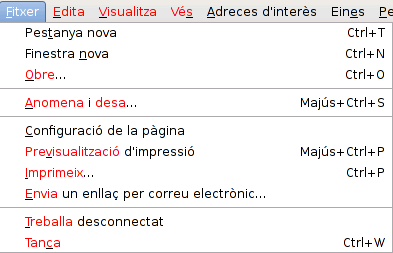
\includegraphics[scale=0.35]{images/epiphany.png}

Captura de pantalla d'un diàleg d'opcions de l'OpenOffice.org amb exemples de l'ús de l'imperatiu en caselles de selecció:

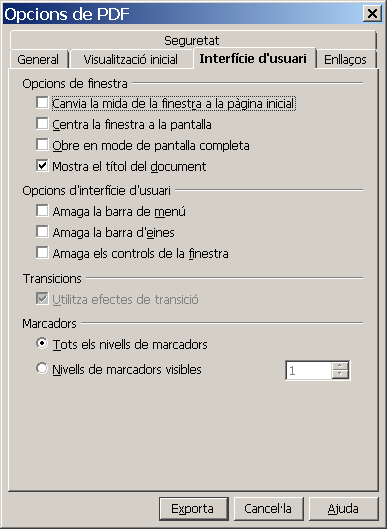
\includegraphics[scale=0.35]{images/openoffice.png}


\cheatsheetsubsection{Gerundi}

Quan en anglès s'utilitza el gerundi per a indicar una acció que s'està executant, en català no s'ha de traduir literalment per un gerundi, sinó que s'ha d'emprar la forma \emph{S'està…} o bé \emph{S'estan…}:

\underline {Text original} Downloading mail.

\underline {No} \textbf{Baixant} el correus.

\underline {Sí} \textbf{S'està baixant} el correu.


\underline {Text original} \textbf{Compacting} databases.

\underline {No} \textbf{Compactant} les bases de dades.

\underline {Sí} \textbf{S'estan compactant} les bases de dades.

\cheatsheetsection{Construccions habituals}

\cheatsheetsubsection{You can}

L'expressió \emph{You can} en anglès es pot usar en el sentit de possibilitat o d'ordre. En el primer cas, cal traduir-la per \emph{podeu} + infinitiu; en el segon, per imperatiu.

Per exemple:

\underline {Anglès} This program is free software; you \emph{can} redistribute it and/or modify.

\underline {Català} Aquest programa és programari lliure; es \emph{pot} redistribuir i/o modificar.

\underline {Anglès} This is a bad idea because as root, you \emph{can} damage your system, and nothing will stop you.

\underline {Català} Això no és recomanable, ja que com a usuari primari \emph{podeu} malmetre el sistema i res no us aturarà.


\cheatsheetsubsection{May}

Habitualment, les construccions amb \emph{may} indiquen possibilitat o bé probabilitat. En el primer cas, les traduirem per \emph{pot} + infinitiu; en el segon, ho farem per \emph{És possible que/pot ser que} + subjuntiu (en cap cas per \emph{pot} + infinitiu). Per exemple:

\underline {Anglès} You \textbf{may} choose individual options to be installed. Recommended for experienced users.

\underline {Català} \textbf{Podeu} triar quines opcions voleu instal·lar. Recomanat només per als usuaris avançats.

Probabilitat:

\underline {Text original} The server \textbf{may be down} or may be incorrectly configured.

\underline {No} El servidor \textbf{pot haver caigut} o estar configurat incorrectament.

\underline {Sí} \textbf{És possible} que el servidor hagi caigut o estigui mal configurat.

A banda dels casos en què expressa possibilitat o probabilitat, el \emph{may} també es fa servir sovint per a fer referència a les característiques o comportament d'alguna cosa.

\cheatsheetsection{Complement + substantiu}

En anglès, el complement va davant el substantiu. Les frases com ara \emph{Operating System Database Manager Program Files} les traduirem cap enrere, és a dir, aquest exemple es traduiria per \emph{Fitxers del programa del gestor de bases de dades del sistema operatiu}.

Sovint és difícil establir si ens trobem davant una construcció del tipus complement + substantiu (com ara \emph{Download Manager}, gestor de baixades), o d'una del tipus verb en imperatiu + substantiu (com ara \emph{Load Settings}, carrega els paràmetres). Només el context ens hi podrà ajudar o, si no n'hi ha, l'experiència en altres casos similars, o fins i tot la intuïció.

D'altra banda, cal recordar que, en català, el complement generalment es posposa al substantiu:

\underline {Text original} Consider following steps:

\underline {No} Tingueu en compte els \textbf{següents} passos:

\underline {Sí} Tingueu en compte els passos \textbf{següents}:


\underline {Text original} New file.

\underline {No} Nou \textbf{fitxer}

\underline {Sí} Fitxer \textbf{nou}.

\cheatsheetsection{L'article}

En anglès no se solen posar els articles \emph{the} ni \emph{a/an} en esmentar determinats conceptes, però en les traduccions al català, i sempre segons el context, en molts casos caldrà afegir-los:

\underline {Text original} Downloading Mail.

\underline {No} S'està baixant correu.

\underline {Sí} S'està baixant \textbf{el} correu.


\underline {Text original} Please select location.

\underline {No} Seleccioneu ubicació.

\underline {Sí} Seleccioneu \textbf{una} ubicació.


\cheatsheetsectiontitle{Aspectes de localització}

\cheatsheetsection{Decimals i milers}

L'ús del punt i la coma com a separadors de decimals i milers canvia segon els països. Per exemple, als Estats Units els milers se separen amb una coma i els decimals amb un punt, mentre que en català, segons les convencions dels principals territoris on es parla, es fa a l'inrevés:

\underline {Anglès} 1,234,567.89 (als Estats Units)

\underline {Català} 1.234.567,89


\cheatsheetsection{Data i hora}

En anglès, les hores s'expressen amb el format de 12 hores (AM o PM); en català, ho farem amb un format de 24 hores i separant l'hora dels minuts i els minuts dels segons per mitjà de dos punts:

Un quart de sis de la tarda, en anglès: \textbf{5:15:00 PM}.

La mateixa hora, en català: \textbf{17:15:00}.

\cheatsheetsubsection{Format i ordre de la data}

El format en què s'expressen les dates depèn de cada país. Als Estats Units, les dates s'expressen com mes/dia/any i en alguns països, com ara Japó, s'expressen com any/mes/dia. En català, utilitzem sempre dia/mes/any (l'any s'escriu sense punt separador de milers):

\underline {Anglès} September 11th, 2000.

\underline {Català}	11 de setembre de 2000.

\cheatsheetsection{Localització de documentació}

\cheatsheetsubsection{Títols}

En anglès, és habitual emprar el gerundi en els títols de seccions de manuals o noms de documents. En català, cal defugir el gerundi i utilitzar preferentment construccions nominals o, si això no és possible, infinitius. Per exemple, traduirem el títol \emph{Adding Graphics to the Gallery} per \emph{Addició de gràfics a la galeria} o, alternativament, \emph{Afegir gràfics a la galeria}.

\cheatsheetsubsection{Referències a opcions de la interfície d'usuari}

Quan traduïm documentació de programari, trobem moltes referències directes a la interfície d'usuari: opcions, botons, funcions, pestanyes. Sovint es tendeix a traduir la documentació sense tenir en compte com es van traduir els mateixos termes en l'aplicació. En conseqüència, una seqüència de passos suggerida pot no coincidir amb les instruccions que cal seguir realment. 

Així doncs, és imprescindible consultar la interfície d'usuari per a assegurar-nos que els passos que es descriuen a la documentació coincideixen exactament amb els que trobem a l'aplicació. Per exemple, si en la documentació es diu que heu d'anar a una opció de menú com ara \emph{Eines > Opcions}, comproveu que la traducció emprada en el programa sigui aquesta.

\cheatsheetsectiontitle{Recursos addicionals}

Guia d'estil de Softcatalà completa:\url{https://www.softcatala.org/guia-estil-de-softcatala/}

Consulteu traduccions prèvies: \url{https://www.softcatala.org/recursos/memories.html}

\cheatsheetfooter{(c)2020 Softcatalà}{https://www.softcatala.org}
\end{multicols*}
\end{document}
